%%%%%%%%%%%%%%%%%%%%%%%%%%%%%%%%%%%%%%%%%%%%%%%%%%%%%%%%%%%%%%%%%%%%%%%%%%%%%%%%
% Project Report Template based on Three Research Papers
% Single Column Format
%%%%%%%%%%%%%%%%%%%%%%%%%%%%%%%%%%%%%%%%%%%%%%%%%%%%%%%%%%%%%%%%%%%%%%%%%%%%%%%%

\documentclass[10pt, a4paper]{article}

% --- PACKAGE SETUP ---
\usepackage[utf8]{inputenc} % For handling text encoding
\usepackage{geometry}       % For setting page margins
\usepackage{amsmath}        % For advanced math typesetting
\usepackage{graphicx}       % For including images
\usepackage{setspace}       % For controlling line spacing (e.g., \onehalfspacing)
\usepackage[
    backend=biber,          % Modern backend for bibliography
    style=authoryear,       % Citation style (e.g., Author, Year)
    sorting=nyt             % Sort references by name, year, title
]{biblatex}
\usepackage{hyperref} 
% \usepackage[margin=1in]{geometry}
\usepackage{amsmath}
\usepackage{amssymb}
\usepackage{graphicx}
\usepackage{float}
\usepackage{caption}
\usepackage{booktabs}
\usepackage{multicol}
\usepackage{lipsum} % For placeholder text if needed
\usepackage{hyperref}
\usepackage{listings}
\usepackage{xcolor}
% For creating hyperlinks in the document (TOC, citations)

% --- DOCUMENT CONFIGURATION ---

% Set page margins
\geometry{a4paper, margin=1in}

% Set line spacing (uncomment the one you need)
\onehalfspacing
%\doublespacing

% Hyperlink setup for a clean look
\hypersetup{
    colorlinks=true,
    linkcolor=blue,
    filecolor=magenta,      
    urlcolor=cyan,
    citecolor=red,
}

% Point to your bibliography file
\addbibresource{references.bib}

% --- TITLE PAGE INFORMATION ---
% <-- EDIT YOUR DETAILS HERE

% --- END OF PREAMBLE ---


\begin{document}

% --- CREATE THE TITLE PAGE ---
\begin{titlepage}
    \centering
    \vspace*{\stretch{1.0}}
    {\Huge \bfseries A Study and Comparative Analysis of Key Research in \\ \vspace{0.5em} \LARGE From Team Centrality to Energy-Efficient Network Control \par}
    \vspace{2cm}
    {\Large Srinjoy Chakraborty \\ 
    251040638\\
    \texttt{srinjoyc25@iitk.ac.in} \par}
    \vspace{1cm}
    
    A report submitted in partial fulfillment of the requirements for the course
    \\[0.5cm]
    {\large \bfseries EE698V: Graph Theory}
    \\[1cm]
    
    Submitted to:
    \\
    {\large Prof. Twinkle Tripathy}
    
    \vspace{1cm}
    {\large 
\includegraphics[width=0.3\textwidth]{redlogo.jpg}} % Optional: Add your university logo
    \\[1cm]
    {\large Electrical Engineering}
    \\
    {\large Indian Institute of Technology, Kanpur}
    \\
    {\large Kanpur, Uttar Pradesh, India}
    \\[1cm]
    
    {\large \today \par}
    \vspace*{\stretch{1.0}}
\end{titlepage}

% --- TABLE OF CONTENTS ---
\tableofcontents
\newpage

% --- MAIN REPORT SECTIONS ---

\section{Introduction}

\subsection*{Background}
The study of complex networks is a cornerstone of modern graph theory, providing a mathematical framework to understand systems ranging from social collaborations to biological processes and engineered infrastructures. A central challenge in this field is to move beyond simple topological descriptions to a deeper understanding of how a network's structure governs its dynamic behavior and function. Classical graph metrics often fall short in capturing the nuances of real-world systems, which frequently involve higher-order interactions (i.e., groups or teams) and are subject to external control. This necessitates the development of more sophisticated analytical tools that can accurately model group influence and quantify the practical costs associated with controlling network dynamics.

\subsection*{Problem Statement and Objective}
The goal of this report is to analyze, compare, and synthesize the findings of three key research papers that bridge the gap between structural graph theory and the control of complex networks. We explore the evolution of centrality measures from individuals to teams, the connection between network topology and the energetic cost of control, and the role of fundamental matrix properties in designing optimal control strategies. By examining these works in concert, we aim to build a cohesive narrative from the problem of measuring influence to the challenge of implementing it efficiently.

\subsection*{Introduction to the Papers}
The report focuses on the following three papers:
\begin{enumerate}
    \item \textbf{Lee et al. (2021), ``Betweenness centrality of teams in social networks'':} This paper addresses the limitation of classical centrality measures by extending the concept of betweenness centrality from individual nodes to teams. It introduces a weighted hypergraph model that accurately represents group collaborations and reveals that team influence is a complex function of both performance and the structural embedding of its members.
    
    \item \textbf{Bof et al. (2017), ``On the Role of Network Centrality in the Controllability of Complex Networks'':} This work moves beyond the binary concept of controllability to analyze the energy required for control. It establishes a formal link between a network's energetic controllability and its structural heterogeneity, as measured by the distribution of eigenvector centrality. This leads to a powerful distinction between ``isotropic'' (homogeneous, hard to control) and ``anisotropic'' (heterogeneous, easier to control) networks.
    
    \item \textbf{Lindmark \& Altafini (2021), ``Centrality Measures and the Role of Non-Normality for Network Control Energy Reduction'':} This paper resolves the conflict between different control energy metrics by introducing network non-normality as a unifying principle. It defines novel centrality measures for a node's influence ($p_i$) versus its reachability ($q_i$) and shows that their imbalance provides a robust and effective strategy for selecting optimal driver nodes.
\end{enumerate}

\subsection*{Structure of the Report}
Section 2 of this report provides a detailed summary and analysis of the hypergraph centrality model. Section 3 explores the link between network centrality and energetic controllability. Section 4 delves into the role of non-normality for optimal driver node selection. Section 5 presents a comparative analysis, synthesizing the key themes across the three works, and Section 6 concludes the report.


\section{Introduction: The Limits of Pairwise Centrality}
The classical measure of a node's influence as a communication broker is its vertex betweenness centrality (v-BC) :
\begin{equation}
    B(v_i) = \sum_{s \neq v_i \neq t} \frac{\sigma_{st}(v_i)}{\sigma_{st}}
\end{equation}
where $\sigma_{st}$ is the number of shortest paths between nodes $s$ and $t$. This definition, however, is fundamentally node-centric. In many real-world social networks, the primary unit of interaction is not an individual, but a team.

A standard graph model $G=(\mathcal{V}, \mathcal{E})$ with $\mathcal{E} \subseteq [\mathcal{V}]^2$ fails to capture this. A single team collaboration (a hyperedge $h \subseteq \mathcal{V}$) and a set of all pairwise interactions between its members (the edge set of a clique, $[h]^2$) are indistinguishable, as both project to a $K_{|h|}$ subgraph. This representational ambiguity necessitates a more expressive framework.

\subsection{Methodology: Hyperedge Betweenness Centrality (h-BC)}

\paragraph{\textbf{Hypergraph Representation:}}
To accurately model group interactions, the network is represented as a hypergraph $\mathcal{H} = (\mathcal{V}, \mathcal{E})$, where $\mathcal{V}$ is the set of individuals and $\mathcal{E}$ is a multiset of hyperedges, each representing a team.

\subsubsection{Bipartite Graph Projection}
\label{{sec:projection}}
The core analytical tool is the projection of the hypergraph onto a bipartite graph $\mathcal{G}_B = (\mathcal{V} \cup \mathcal{E}, E_B)$. The two partitions of the vertex set are the individuals ($\mathcal{V}$) and the teams-as-nodes ($\mathcal{E}$). The edge set is formally defined as:
\begin{equation}
    E_B = \{ \{v, e\} \mid v \in \mathcal{V}, e \in \mathcal{E}, \text{ and } v \in e \}
\end{equation}
This structure provides a tractable model for applying pathfinding algorithms.

\subsubsection{Weighted Shortest Paths}
A path between two individuals $s,t \in \mathcal{V}$ is an alternating sequence of nodes from $\mathcal{V}$ and $\mathcal{E}$ in $\mathcal{G}_B$. In an unweighted model, the sheer number of such paths dilutes centrality scores, masking the influence hierarchy. To resolve this, a cost $c_i$ is assigned to each hyperedge $e_i$. The paper explores two performance metrics for weighting:
\begin{itemize}
    \item \textbf{Team Performance ($u_i$):} An empirical value, e.g., the number of articles a team published.
    \item \textbf{Performance per Member ($w_i$):} A normalized value, $w_i = u_i / |e_i|$.
\end{itemize}
The cost is the inverse of a performance metric, e.g., $c_i = 1/u_i$. A shortest path is one that minimizes the total cost, $L(P_{st}) = \sum_{e_i \in P_{st}} c_i$.

\subsubsection{Formal Definition of h-BC}
The Hyperedge Betweenness Centrality (h-BC) of a team $e$ is its betweenness centrality score within the weighted bipartite graphr or its the projection of the bipartitte graph as discussed in section \ref{sec: projection} $\mathcal{G}_B$:
\begin{equation}
    B_H(e) = \sum_{s,t \in \mathcal{V}, s \neq t} \frac{\sigma_{st}(e)}{\sigma_{st}}
\end{equation}
where $\sigma_{st}$ is the number of shortest-cost paths. 
\subsection{Citation network vs Hypergraph}
\paragraph{Why betweenness centrality matters more than degree centrality here:} 
First, it's important to clarify that our model is a co-authorship network, where authors are nodes and papers are hyperedges. This is different from a basic citation network, where nodes are papers.

In this co-authorship model, betweenness centrality and degree centrality measure fundamentally different things and answer different questions.


\begin{figure}[h]
    \centering
    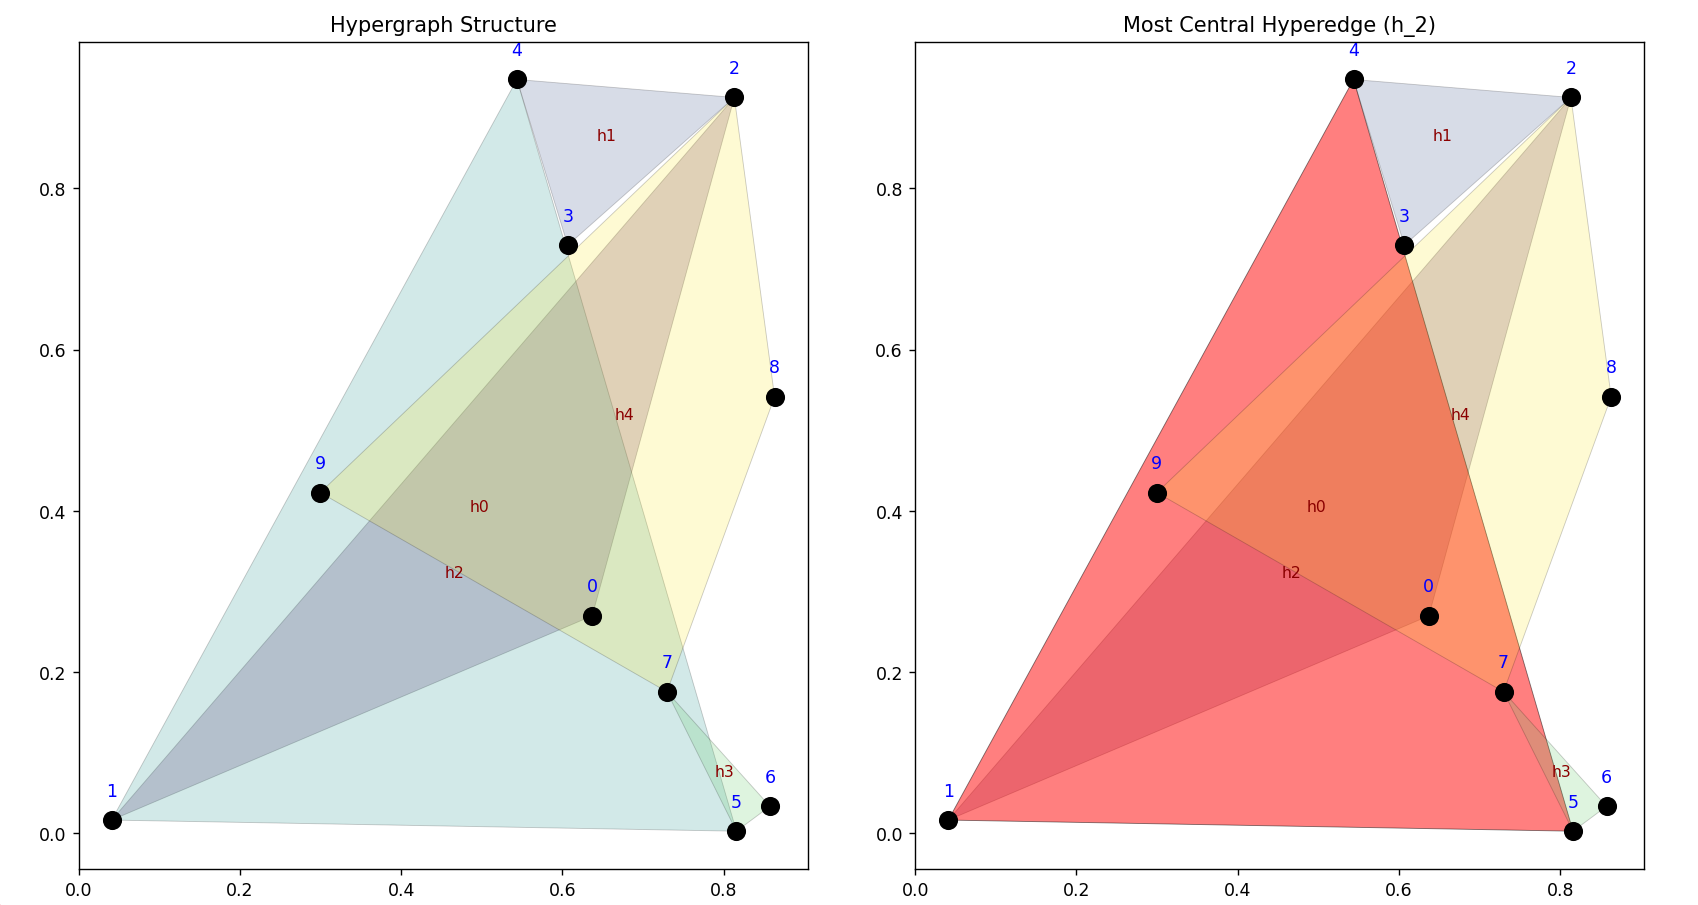
\includegraphics[width=1\linewidth]{hypergraph.png}
    \caption{Hypergraph Model}
    \label{fig:hypergraph}
\end{figure}
\begin{itemize}
    \item What Each Metric Measures in our Authorship Model
    \begin{itemize}
    \item \textbf{Hyperdegree Centrality (Degree Centrality):}
This measures the number of collaborations an individual author is involved in. It is a local measure of an author's activity or collaborative breadth. In our example:
Node 2 is the most degree-central author with a hyperdegree of 3.
This tells us that Author 2 is the most active collaborator.
    \item \textbf{Hyperedge Betweenness Centrality (h-BC):}
This measures how often a team (i.e., a paper) lies on the most efficient paths for information to flow between all pairs of authors in the network. It is a global measure of a collaboration's importance as a bridge. In our example, the team $h_2=1,4,5$ is the most central.
\end{itemize}
    \item \textbf{Why not just use degree centrality?}
Knowing that Author 2 is the most active collaborator (highest degree) is useful, but it doesn't tell us which of their projects was the most impactful for the network's cohesion. It can't distinguish team importance: Does Author 2's presence make team $h_0, h_1, or  h_4$ the most important bridge? Degree centrality alone cannot answer this. It assigns importance to the person, not the project.It's a poor proxy for bridge-like roles: A high-degree node might connect many people who are already well-connected to each other. This makes the node an active hub, but not necessarily a critical bridge between otherwise disconnected communities.
    \item \textbf{Why betweenness centrality is the right tool for this?}
Science and collaboration are not just about individual activity; they are about the synthesis and transfer of ideas between different groups. Betweenness centrality is the only measure that directly quantifies this role.
In your specific example, betweenness centrality correctly identified that the collaboration $h_2=1,4,5$ is the most influential. Why? Because it serves as an essential intellectual bridge. Author 1 is from the orbit of team $h_0$, Author 4 is from team $h_1$, and Author 5 is from team $h_3$.
The project $h_2$ is the one and only place where these three distinct research clusters are directly and efficiently linked.
Degree centrality would have missed this completely. It would have pointed to Author 2, but it wouldn't have revealed that the specific project $h_2$ was the most critical event for the overall cohesion and information flow of the entire research community.

\end{itemize}











% \section{Conclusion}
% The hypergraph betweenness centrality provides a necessary and powerful extension to classical network theory. By accurately modeling group interactions and employing a weighted pathfinding approach, it successfully quantifies the influence of teams as single, cohesive entities. The framework reveals that team influence is a nuanced property, emerging from an interplay between the team's performance, its structural position as a bridge, and the connectivity of its individual members. This methodology offers a more realistic tool for analyzing a wide range of social, biological, and technological systems where collaboration is key.




\section{The limits of Classical Controlability}
The classical notion of controllability mainly dwells in a binary approach: a network is either controllable or not! This approach however, is often based on structural controllability, which is trivial for determining the minimum number of control nodes to ensure control is theoretically as well as practically possible. A network may be controllable on paper but require physically unrealizable amounts of energy, making it "practically uncontrollable". The goal of this research was to establish a formal link between the network's graphical topology and this control energy cost.
\subsubsection{Control Energy Shift}
They modeled the network as a discrete-time Linear Time-Invariant (LTI) system :
\begin{equation}
    x(t+1) = Ax(t) + B_{\mathcal{K}}u_{\mathcal{K}}(t)
    \label{eq:lti}
\end{equation}
Where $x(t) \in \mathbb{R}^n$ is the state vector, $A \in \mathbb{R}^{n \times n}$ is the network's adjacency matrix, and $B_{\mathcal{K}}$ is an input matrix selecting $m$ control nodes from the set $\mathcal{K}$ . The energy needed for control is fundamentally linked to the Controllability Gramian, defined as :
\begin{equation}
    W_{\mathcal{K},T} = \sum_{\tau=0}^{T-1}A^{\tau}B_{\mathcal{K}}B_{\mathcal{K}}^{\top}(A^{\top})^{\tau}
    \label{eq:gramian}
\end{equation}
To quantify control difficulty, we analyze the worst-case energy required to steer the system. This is given by the inverse of the smallest eigenvalue of the Gramian, $\lambda_{\min}(W_{\mathcal{K},T})$. A system is considered difficult to control if $\lambda_{\min}(W_{\mathcal{K},T})$ is very small.
\subsubsection{Assumptions and analysis}
The analysis relies on the spectral properties of the network matrix $A$.

\paragraph{Assumption 1:} \label{sec:assumpt1} The network matrix $A$ is irreducible and marginally stable. This guarantees a unique, real principal eigenvalue $\lambda_1 = \rho(A)$ such that $1 \ge \lambda_1 \ge |\lambda_i|$ for all other eigenvalues $\lambda_i$ of $A$.

This assumption ensures the existence of strictly positive right ($v$) and left ($w$) leading eigenvectors corresponding to $\lambda_1$ {1983}:
\begin{equation}
    Av = \lambda_1 v, \quad A^{\top}w = \lambda_1 w
    \label{eq:eigenvectors}
\end{equation}
From these, we construct a related symmetric, positive semi-definite matrix $A_S$ as follows:
\begin{equation}
    \pi= [\frac{w_1}{v_1}\frac{w_2}{v_2} ...\frac{w_n}{v_n}]^{\top}
\end{equation}
The diagonal matrix: \\
\begin{equation}
\Pi:= \text{diag}(\pi) \\
,A_R:= \Pi^{-1}A^{\top}\Pi \quad  \\
\end{equation}
The matrix $A_R$  is irreducible and $v,w$ are its leading eigen vectors with respect to $\lambda_1$.
\begin{equation}
A_S:= \Pi^{1/2} A A_R \Pi^{-1/2}
\end{equation}
Let the eigenvalues of $A_S$ be sorted as $\sigma_1 \ge \sigma_2 \ge \dots \ge \sigma_n \ge 0$. The largest eigenvalue is $\sigma_1 = \lambda_1^2$.
\subsection{Results}

\subsubsection{A Structural Bound on Control Energy}
The main result from provides a direct link between the network's structural properties (encoded in its eigenspace) and its energetic controllability.

\paragraph{Theorem 1:} Let $A$ be a non-negative matrix satisfying Assumption 1, as in section \ref{sec:assumpt1}, and assume the product $AA^{\top}$ is primitive. The minimum eigenvalue of the controllability Gramian for any set $\mathcal{K}$ of $m$ control nodes is bounded by:
% \begin{equation}
%     % \lambda_{\min}(W_{\mathcal{K},T}) \le \frac{\max_{i}\{w_{i}/v_{i}\}}{\min_{i}\{w_{i}/v_{i}\}}\frac{\sigma_{2}^{\frac{n}{m}-2}}{1-\sigma_{2}}
%     % \label{eq:main_bound}
%     \lambda_{\min}(W_{\mathcal{K},T}) \le \frac{\max_{i}\{w_{i}/v_{i}\}}{\min_{i}\{w_{i}/v_{i}\}}\frac{\sigma_{2}^{\frac{n}{m}}{\sigma_2^2(1-\sigma_2)}
% \end{equation}
\begin{equation}
    \lambda_{\min}(W_{\mathcal{K},T}) 
    \le 
    \underbrace{
        \frac{\max_{i}\left\{\frac{w_{i}}{v_{i}}\right\}}{\min_{i}\left\{\frac{w_{i}}{v_{i}}\right\}}
    }_{\text{anisotropy ratio}}
    \cdot
    \underbrace{
        \frac{\sigma_{2}^{\frac{n}{m} }}{\sigma_2^2(1 - \sigma_{2})}
    }_{\text{spectral properties}}
    \label{eq:main_bound}
\end{equation}


This bound shows that control difficulty depends on the anisotropy ratio (the first term, measuring structural imbalance) and the spectral properties of the network (the second term, related to the mixing rate).
\subsubsection{Case of Reversible Matrices}
The interpretation becomes even more concrete for the subclass of reversible stochastic matrices. A stochastic matrix is reversible if it satisfies $A=A^R$, where $A^R$ is the time-reversal matrix defined in Equation \ref{eq:ar}. This class includes the transition matrices of random walks on undirected graphs.

For a random walk on an undirected graph with a symmetric adjacency matrix $C$, the transition matrix is $A=CD^{-1}$. In this case, the eigenvector centrality $v_i$ is directly proportional to the weighted degree of the node:
\begin{equation}
    v_i = \frac{C_{i}^{\text{col}}}{C_{\text{tot}}} = \frac{\sum_{j}C_{ji}}{\sum_{i,j}C_{ij}}
\end{equation}
This establishes a direct link between the abstract eigenvector centrality and the simple, intuitive graph property of node degree. Consequently, the heterogeneity index simplifies to the ratio of the maximum to minimum degree:
\begin{equation}
    \frac{v_{\max}}{v_{\min}} = \frac{\max_{i}\{C_{i}^{\text{col}}\}}{\min_{i}\{C_{i}^{\text{col}}\}}
\end{equation}
\subsubsection*{The Perron-Frobenius Theorem and Its Link to the Paper}
The Perron-Frobenius theorem applies to any non-negative, \textbf{irreducible} matrix $A$ (which represents a strongly connected graph). It guarantees:
\begin{itemize}
    \item A unique, real, and positive eigenvalue $\lambda_1$ that is equal to the spectral radius of the matrix, $\lambda_1 = \rho(A)$.
    \item Corresponding left ($w$) and right ($v$) eigenvectors that are \textbf{strictly positive}, meaning all their components are positive.
\end{itemize}

\paragraph{Its Crucial Role in the Paper}

The paper's analysis is entirely dependent on these guarantees:

\begin{itemize}
    \item \textbf{It Establishes Centrality Vectors}: The theorem ensures that the vectors $v$ and $w$---which the paper interprets as \textbf{eigenvector centrality}---exist, are unique (up to scaling), and are positive for any connected network.Without this, the core concept of a heterogeneity index ($\frac{v_{\max}}{v_{\min}}$) would be ill-defined.

    \item \textbf{It Enables the Entire Framework}: All subsequent mathematical objects in the paper, including the anisotropy ratio, the time-reversal matrix $A^R$, and the symmetric matrix $A_S$, are constructed directly from these guaranteed positive eigenvectors $v$ and $w$.
\end{itemize}

In essence, the Perron-Frobenius theorem provides the necessary starting point, allowing the authors to confidently extract well-defined centrality vectors from the network's structure, which is the first and most critical step in their entire analysis of control energy.
\subsubsection{From $\sigma_2$ to the Controllability Metric ($\lambda_{\min}(W)$)}
This final step connects the structural parameter $\sigma_2$ to the ultimate measure of control difficulty using the paper's main theorem \ref{eq:main_bound}.
We begin with the paper's Theorem 1 \ref{eq:main_bound}, which states that the controllability metric is constrained by an upper bound involving $\sigma_2$. For the case of an undirected graph (where the anisotropy ratio becomes the heterogeneity index), the bound is:
\begin{equation}
    \lambda_{\min}(W_{\mathcal{K},T}) \le \frac{v_{\max}}{v_{\min}}\frac{\sigma_{2}^{\frac{n}{m}-2}}{1-\sigma_{2}}
\end{equation}
\paragraph{Substituting the Expression for $\sigma_2$}
for a reversible matrix (like a random walk on an undirected graph), $\sigma_2$ is determined by the eigenvalues of the transition matrix $A$:
\begin{equation}
    \sigma_2 = \max\{\lambda_2(A)^2, \lambda_n(A)^2\}
\end{equation}
Also we have the crucial link to the algebraic connectivity:
\begin{equation}
    \lambda_2(A) = 1 - \mu_2(L_{norm})
\end{equation}
We can now substitute these relationships directly into the main theorem's inequality Eq.(\ref{eq:main_bound}). This gives us a single, comprehensive expression that explicitly links the algebraic connectivity of the graph Laplacian to the controllability bound:
\begin{equation}
    \lambda_{\min}(W) \le \frac{v_{\max}}{v_{\min}} \frac{ \left( \max\{(1-\mu_2(L_{norm}))^2, \lambda_n(A)^2\} \right)^{\frac{n}{m}-2} }{ 1 - \max\{(1-\mu_2(L_{norm}))^2, \lambda_n(A)^2\} }
\end{equation}
\paragraph{Mathematical Interpretation}
This expression, while complex, formally demonstrates the complete mathematical chain and allows us to analyze the relationship:
\begin{itemize}
    \item A high algebraic connectivity (a large $\mu_2(L_{norm})$) makes the term $(1-\mu_2(L_{norm}))$ smaller.
    \item This, in turn, leads to a small $\sigma_2$, as long as the smallest eigenvalue $\lambda_n(A)$ is not close to $-1$.
    \item A small $\sigma_2$ has two beneficial effects on the bound:
    \begin{enumerate}
        \item It makes the denominator $1-\sigma_2$ large.
        \item It makes the numerator, which contains $\sigma_2$ raised to a positive power (for $n>2m$), small.
    \end{enumerate}
\end{itemize}
Both of these effects push the upper bound on $\lambda_{\min}(W)$ higher. A higher bound means the system is permitted to have better controllability.

\vspace{1em}
\noindent Therefore, the structural cohesion of the graph, as measured by the algebraic connectivity ($\mu_2(L_{norm})$), propagates through the spectral properties of the system's transition matrix to place a hard, quantifiable limit on its energetic controllability ($\lambda_{\min}(W)$).
\paragraph{Inference from the Simulation Result}
\begin{figure}[h]
    \centering
    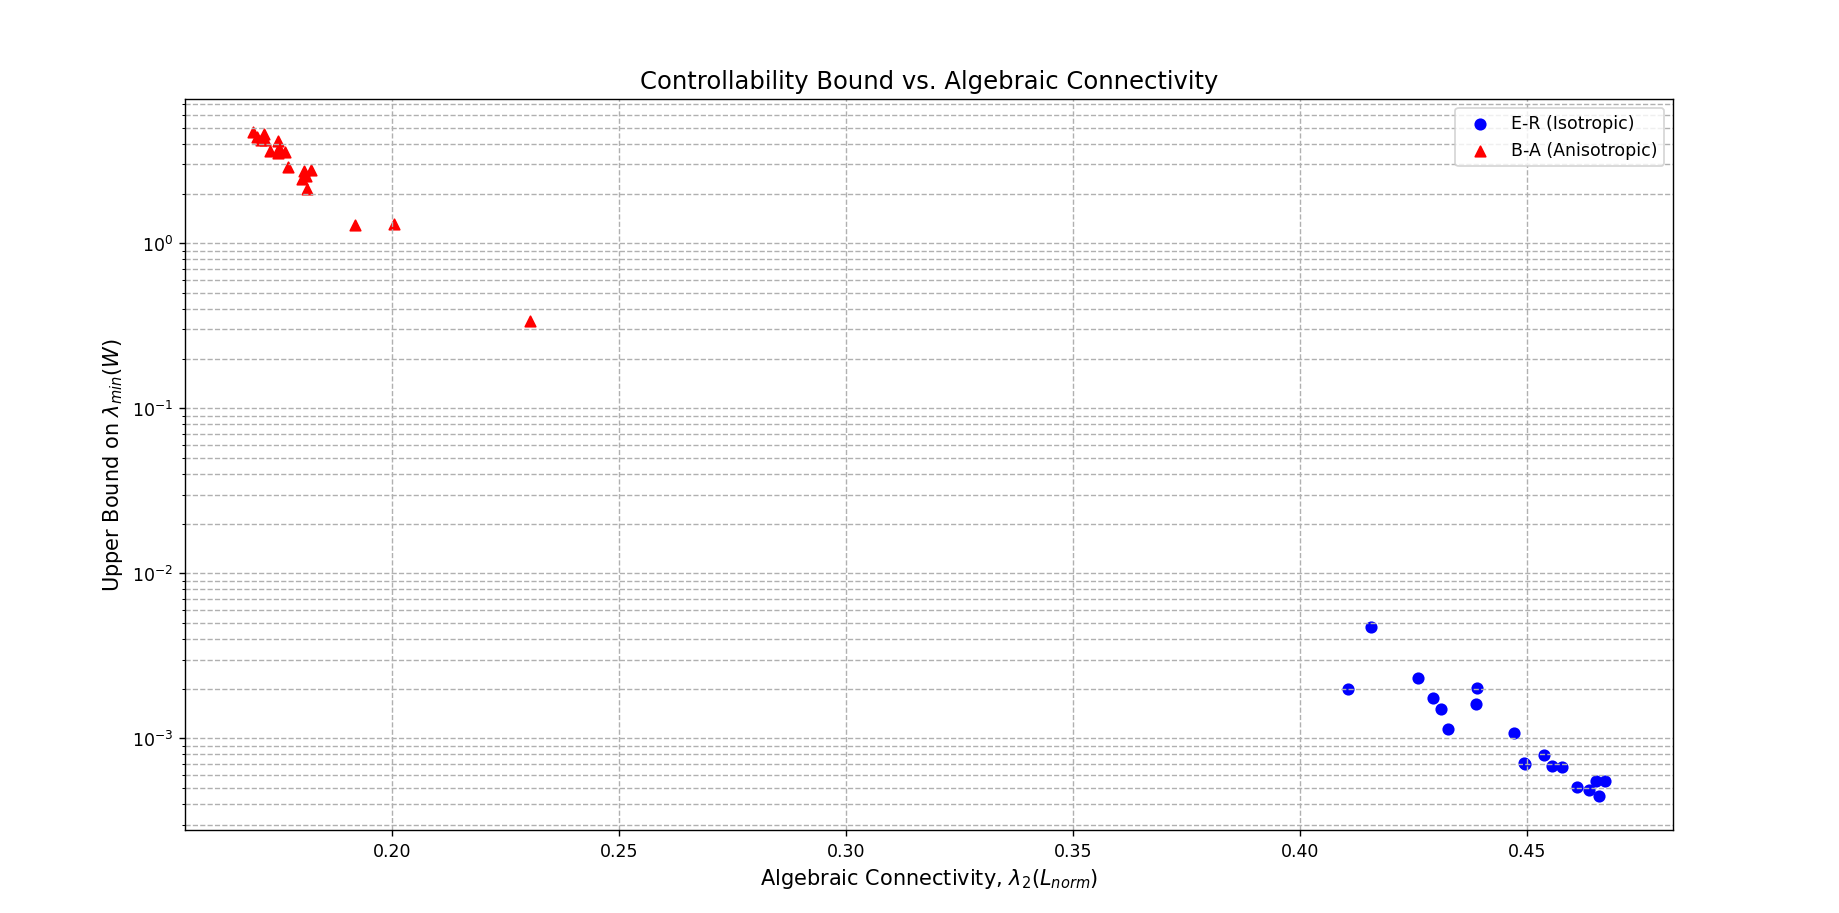
\includegraphics[width=1\linewidth]{sim.png}
    \caption{Upperbound and cohesion relation}
    \label{fig:sim_result}
\end{figure}
The simulation plot Figure:  visually confirms  this relationship, but adds a crucial nuance:
The E-R (Isotropic) graphs (blue circles) have high algebraic connectivity but a very low controllability bound. Their structural uniformity makes them difficult to control. The B-A (Anisotropic) graphs (red triangles) have a much higher controllability bound, even with lower algebraic connectivity. Their structural heterogeneity is the dominant factor.
The key takeaway is that while structural cohesion is important, the diversity of node influence (anisotropy) is the more critical factor for achieving energy-efficient control in complex networks.
\section{Resolving the Dilemma with Non-Normality}
The choice of driver nodes presents a dilemma: maximizing average efficiency ($Tr(W)$) favors influential hubs, while minimizing worst-case energy ($\lambda_{\min}(W)$) favors hard-to-reach nodes . This conflict is resolved by analyzing the network's non-normality.
A matrix is normal if it commutes with its transpose, $[A, A^\top] = 0$ . The paper proves that a network is a balanced realization (where controllability and observability are balanced) if and only if $A$ is normal. Non-normality can be quantified at the node level by defining two novel centralities based on "walk energy" $\epsilon_{i \to j}$:

\begin{itemize}
    \item \textbf{Node-to-Network ($p_i$)}: Measures influence.
    \begin{equation}
        p_i = \sum_{j=1}^{n} \epsilon_{i \to j} = Tr(W^{(i)}) \quad 
    \end{equation}
    \item \textbf{Network-to-Node ($q_j$)}: Measures reachability.
    \begin{equation}
        q_j = \sum_{i=1}^{n} \epsilon_{i \to j} = Tr(M^{(j)}) \quad 
    \end{equation}
\end{itemize}
Node-level non-normality is then the imbalance between these two:
\begin{equation}
    r_{\text{diff},i} = p_i - q_i \quad 
\end{equation}


\subsection{Case Study: Optimal Driver Node Selection}
We now apply this theory to the 6-node network from Figure , implemented by the Python code .

% \begin{figure}[H]
%     \centering
%     \includegraphics[width=0.9\linewidth]{network_graph.png}
%     \caption{The 6-node directed graph for the case study.}
%     \label{fig:network_case_study}
% \end{figure}

\begin{table}[H]
    \centering
    \caption{Centrality and Non-Normality Measures for the 6-Node Network.}
    \label{tab:centrality_case_study}
    \begin{tabular}{@{}ccccc@{}}
        \toprule
        \textbf{Node} & \textbf{p (Infl.)} & \textbf{q (Reach.)} & \textbf{r\_diff} & \textbf{r\_quot} \\ \midrule
        1 & 0.76 & 0.50 & 0.26 & 1.52 \\
        2 & 0.82 & 0.71 & 0.11 & 1.15 \\
        3 & 0.64 & 0.50 & 0.14 & 1.27 \\
        4 & 0.90 & 0.73 & 0.17 & 1.23 \\
        5 & 0.53 & 0.86 & -0.33 & 0.62 \\
        6 & 0.57 & 0.91 & -0.34 & 0.63 \\ \bottomrule
    \end{tabular}
\end{table}

\begin{table}[H]
    \centering
    \caption{Performance of Driver Selection Strategies {2127-2146}.}
    \label{tab:performance_case_study}
    \begin{tabular}{@{}lccc@{}}
        \toprule
        \textbf{Driver Set} & \textbf{$Tr(W)$} & \textbf{$\lambda_{\min}(W)$} & \textbf{$Tr(W^{-1})$} \\ \midrule
        $\{2,4\}$ (Max $p_i$) & 1.72 & 0 & $\infty$ \\
        $\{1,4\}$ (Max $r_{\text{diff}}$) & 1.66 & $3.84 \cdot 10^{-5}$ & $2.80 \cdot 10^4$ \\
        $\{1,3\}$ (Max $r_{\text{quot}}$) & 1.39 & $1.11 \cdot 10^{-3}$ & $1.04 \cdot 10^3$ \\ \bottomrule
    \end{tabular}
\end{table}

The results in Table \ref{tab:performance_case_study} are stark. The naive strategy of maximizing influence ($\mathcal{K}_{Tr}=\{2,4\}$) fails catastrophically, rendering the system uncontrollable ($\lambda_{\min}=0$) because it neglects the root node (Node 1). The non-normality strategies succeed by selecting nodes with high imbalance (like Node 1), ensuring controllability and providing a robust trade-off between average and worst-case energy.

% \section{Conclusion}
% The research presented provides a powerful narrative, moving from the abstract spectral properties of a network's adjacency matrix to a practical, effective strategy for control. The key insight is that the structural heterogeneity of a network, quantifiable via centrality measures, directly governs the energy required for its control. The concept of non-normality provides a unifying principle that resolves the conflict between competing energy metrics, leading to robust driver node selection strategies. This work elegantly demonstrates how deep concepts from graph theory are essential for solving complex problems in the engineering of networked systems.

\section{Comparative Analysis and Synthesis}

This section provides a comparative analysis of the three papers, connecting their methodologies, results, and overarching themes to build a cohesive understanding of the relationship between network structure and function.

\subsection{Comparison of Methodologies}
The approaches in the three papers represent a clear progression from structural representation to dynamic analysis.
\begin{itemize}
    \item \textbf{Lee et al. (2021)} employs a primarily \textbf{combinatorial and structural} methodology. The core research here in this case is the re-definition of the network model itself from a standard graph to a hypergraph, which is then projected onto a bipartite graph. The analysis considers a common co-authorship model, and betweenness centrality as a metric, but here in this case, BC is applied to a group/ team setup, not on individual vertices

    \item \textbf{Bof et al. (2017)} shifts the focus to \textbf{control theory and linear algebra}. It takes the standard graph representation (the adjacency matrix $A$) as given and uses it as a state space parameter for LTI systems. The metrics which are used are not path-based, but are derived from the system's Controllability Gramian and its $\lambda_{\min}(W)$, eigenspace of $A$.
    
    \item \textbf{Lindmark \& Altafini (2021)} builds directly on the  dynamical systems approach of \cite{Bof2017Role}. Its methodology is also rooted in control theory, using Gramians and $\mathcal{H}_2$ norms. Its primary innovation is the definition of novel centrality measures ($p_i, q_i$) derived directly from energy-based integrals, and using their imbalance to quantify the matrix property of non-normality.
\end{itemize}
In essence,\cite{Lee2021Betweenness} change the graph to better fit the problem, while \cite{Bof2017Role} \& \cite{Lindmark2021Centrality}apply a dynamic lens to analyze the standard graph structure.

% \subsection{Comparison of Results}
% The findings of the three papers are not contradictory; rather, they are complementary and build upon one another in a logical sequence, specially the papers build upon the notion of Controllability Gramian.
% \begin{itemize}
%     \item The result from \textbf{Lee et al.} that a team's influence is strongly correlated with a ``super leader'' (a member with high hyperdegree) highlights that certain nodes are structurally more important for the network's global connectivity.
    
%     \item The work of \textbf{Bof et al.} provides a dynamic consequence for this structural observation. It proves that a network with a high diversity of node importance (anisotropy, measured by eigenvector centrality) is energetically easier to control. The ``super leaders'' identified by Lee et al. are the nodes that create this beneficial anisotropy.
    
%     \item \textbf{Lindmark \& Altafini} provide the most refined perspective. They agree that influential nodes are important but show that a strategy based solely on influence is flawed. Their results demonstrate that the optimal strategy involves selecting nodes based on the \textit{imbalance} between their influence ($p_i$) and their own reachability ($q_i$). This explains why a ``super leader'' (high influence) who is also a root node (low reachability) is an ideal driver node.
% \end{itemize}

\subsection{Common Themes}
Several overarching themes connect all three papers:
\begin{enumerate}
    \item \textbf{Beyond Local Metrics:} All three works argue that simple, local metrics like degree centrality  are insufficient for understanding complex network phenomena as discussed by \cite{Lee2021Betweenness}. They all propose more sophisticated, globally-aware measures: hypergraph betweenness centrality, eigenvector centrality, and energy-based non-normality metrics.
    
    \item \textbf{The Importance of Heterogeneity:} A central theme is that non-uniformity is not noise but a key feature. \cite{Bof2017Role} explicitly frame this as anisotropy. \cite{Lee2021Betweenness} observe it in the power-law distribution of influence driven by super leaders. \cite{Lindmark2021Centrality} leverage it via non-normality. In all cases, a heterogeneous, hierarchical structure has profound and often beneficial effects on the network's function.
    
    \item \textbf{Structure Dictates Dynamics:} This is the most fundamental theme. The static graph topology—who is connected to whom, and in what configuration—has direct, quantifiable consequences on dynamic processes like information flow and the energetic cost of control.
\end{enumerate}

\subsection{Research Gaps and Limitations}
Despite their contributions, the papers point towards several open questions:
\begin{itemize}
    \item The models in Bof et al. and Lindmark \& Altafini are for Linear Time-Invariant (LTI) systems. A major challenge is extending these principles to the \textbf{non-linear dynamics} that govern many real-world biological and social systems.
    \item The Bof et al. paper provides an upper bound on control energy and shows that isotropy makes networks hard to control. The full converse—whether high anisotropy \textit{guarantees} a network is easy to control—remains an open question.
    \item All three analyses assume a complete and accurate knowledge of the network topology. A significant practical challenge is the analysis and control of networks with \textbf{incomplete, uncertain, or time-varying} data.
\end{itemize}

\section{Conclusion}
\subsection{Summary of Analysis}
The progression across these three papers illustrates a clear intellectual journey. It begins with the need for better structural models to understand influence (hypergraphs), moves to linking network structure to dynamic properties like control energy (anisotropy), and culminates in a sophisticated principle (non-normality) that resolves a key practical dilemma in control strategy. The key takeaway is that effective network analysis requires moving beyond local, static metrics to global, dynamic, and often counter-intuitive principles that embrace the inherent heterogeneity of complex systems.

\subsection{Broader Implications}
The research has significant implications for the design and management of a wide range of real-world systems. The principles discussed can inform strategies for enhancing the robustness of communication networks and power grids, designing therapeutic interventions in biological networks by targeting key protein complexes, and understanding the flow of influence in social and economic networks.

\subsection{Future Directions}
Based on the identified gaps, interesting directions for future work include extending the energy-based control framework to non-linear dynamics, developing a more complete theory for the sufficiency of anisotropy in ensuring controllability, and creating new algorithms for network analysis and control that are robust to incomplete or noisy data.



% --- BIBLIOGRAPHY ---
\printbibliography[title={References}]


\end{document}